\chapter{Design}
\label{Chapter:Design}

This chapter discusses the design considerations during the design stage of the system. This stage of the development is very important since it lays down the foundation for the whole system.
Thus a considerable amount of time has been spent to carefully plan how the system should be designed. \citet[12]{bell2005} states that about 5\% of the total time that takes for the development of a software should be spent for the design state alone. For comparison, the coding process takes about 7\%; Testing takes 8\%. 

The design process has gone through many iterations to ensure the best possible quality of the product. The research presented in chapter \ref{Chapter:Literature-Review} had a major impact on the design. The design can be split into four main sections, namely Mobile Platform and IDE; Database Design; Architectural design; and User Interface (UI).

    

    \section{Mobile Platform and IDE}
    The first point that was considered in the design process was the \textbf{mobile platform} on which the proposed application would be implemented and distributed. After research on the current market, Google's \textit{Android} was found to dominate in Europe \citep{williams2016}. Android-based smartphones hold 75.6\% of market share dominating other mobile platforms such as Apple's \textit{iOS} (18.9\%) and Microsoft's \textit{Windows Phone} (4.9\%). Thus, Android OS was chosen to form the basis of the proposed mobile application since it allows the application to be downloaded and used by as many people as possible. In addition, the platform provides an excellent opportunity to reinforce the target market as sedentary people rather than fitness focused users who may favour Apple.
        
    After choosing the mobile platform, the development environment or the \textbf{Integrated Development Environment} (\gls{ide}) was picked. That was an easy decision since \textit{Android Studio} is known to be the official \gls{ide} for Android development \citep{androidstudio2017}. It provides all the necessary developer tools such as \textit{Android Emulator} which is a basically a virtual phone that allows a developer to test an application on different versions of the platform. In addition, it supports direct integration with \textit{Git} which is the version control system used in this project.
    
    \section{HAR}
    The Human Activity Recognition process involves standard stages such as \textit{Data Preprocessing}, \textit{Feature Extraction} and \textit{Feature Selection} (see section \ref{section:feature-selection&extraction}). The block diagram of the \gls{har} process can be seen in figure \ref{fig:har_process}. It shows the main stages of the \gls{har} process implemented in this project. The raw accelerometer data is segmented into \textit{Time windows}. After that it undergoes the \textit{Data Processing} stage where the data is pre-processed e.g., removing the earth's gravitational force from the data. Next, \textit{Feature Extraction} process abstracts the data into 20 features. The \textit{Feature Selection} process is responsible of reducing the number of the features without compromising the data quality. Finally, the \textit{Classifier} determines what class the recognised activity belongs to (e.g. walking).
    
    Weka\footnote{\url{http://www.cs.waikato.ac.nz/ml/weka/}} Data Mining Software has been chosen for the implementation of the \gls{har} component of the proposed system. Since there is no official support of the Weka API on the Android platform, a stripped-down version\footnote{\url{https://github.com/rjmarsan/Weka-for-Android}} of the original Weka Java API has been chosen. This library was tested prior to the design stage to ensure it functions well on an android device. 
    
    \begin{figure}[H]
        \centering
        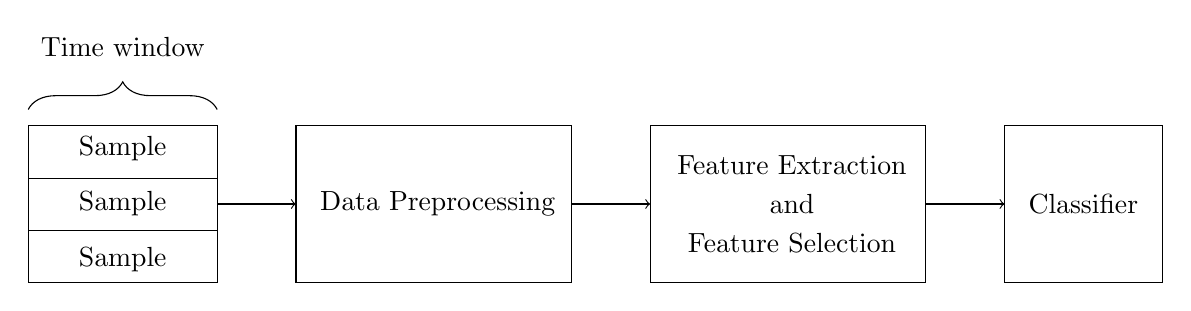
\begin{tikzpicture}
            \node at (1.2,3) {Time window};
            \draw (0,0) rectangle (2.4,2);
            \draw [decorate,decoration={brace,amplitude=10pt}] (0.0,2.2) -- (2.4,2.2); 
            \draw (0,0.66) -- (2.4,0.66);
            \draw (0,1.32) -- (2.4,1.32);
            \node at (1.2,1) {Sample};
            \node at (1.2,0.3) {Sample};
            \node at (1.2,1.7) {Sample};
            \draw [->] (2.4,1) -- (3.4,1);
            \draw (3.4,0) rectangle (6.9,2);
            \node at (5.2,1) {Data Preprocessing};
            \draw [->] (6.9,1) -- (7.9,1);
            \draw (7.9,0) rectangle (11.4,2);
            \node at (9.7,1.5) {Feature Extraction};
            \node at (9.7,1) {and};
            \node at (9.7,0.5) {Feature Selection};
            \draw [->] (11.4,1) -- (12.4,1);
            \draw (12.4,0) rectangle (14.4,2);
            \node at (13.4,1) {Classifier};
        \end{tikzpicture}
        \caption{Human Activity Recognition process}
        \label{fig:har_process}
    \end{figure}
    
    \subsection{Dataset}
    \textit{"Active Minutes"} is using a \textit{Supervised} learning method. This learning method require labeled \textit{"training data"} or \textit{"data set"} in order to build a classifier (or model). After a classifier is build it can be used to classify \textit{"unseen"} or \textit{"unlabelled"} data acquired by the build-in accelerometer sensor in the device.
    
    
    \subsection{Data Processing}
    The data processing stage of \gls{har} normally involves segmenting the data into time windows. Considering the fact that the system will be running on a mobile device with limited resources, the window length has to be picked carefully. For example, choosing a 20-second window length (see figure \ref{fig:har_process}) will cause the CPU to do more work due to the amount of \textit{samples} pulled from the accelerometer sensor in the time window. Consequently, that would lead to a higher battery consumption \citep[2]{torreshuitzil2015a}. As it was found in the literature review (see section \ref{section:learning_alg_accuracy_power_consm}) 3-second time window produces good results in terms of power consumption. Based on those findings, the proposed application will adopt this window length as well.
    
    During this stage, different filters could be applied to the raw data to remove unwanted information. For example, according to \citet[]{googlemotionsensors}, the raw data from an accelerometer sensor contains the earth's gravity force as well. This will cause the device to read magnitude of g = 9.81 m/s2 when it is not accelerating (i.e. laying down on a table). In order to obtain just the linear acceleration without natural forces (i.e. earth's gravitation), a low-pass filter is applied.
    
    In order to reduce the effect of device location (e.g. where the device is ) the magnitude of the accelerometer's x,y and z axis is also calculated during this stage and used as a 4th axis \textit{"m"} (see equation \ref{eq:acceleration_magnitude}). This technique has been used in previous works as well \citep[153]{torreshuitzil2015b}.
    
    \begin{equation}
        \label{eq:acceleration_magnitude}
        m = \sqrt{x^2 + y^2 + z^2}
    \end{equation}
    
    \subsection{Feature Extraction and Feature Selection}
    \textbf{Feature extraction} is an important process in a \gls{har} system. It allows extracting key characteristics from raw data which can be used to represent important patterns with reduced dimensionality \citep[154]{torreshuitzil2015b}. During the initial research (see section \ref{section:feature-selection&extraction}) it was found that extracting the first \gls{fft} algorithm coefficients produce higher accuracy compared to the other features (e.g. Time domain features such as Mean or Standard Deviation). To ease the development process, a third-party library called \textit{JTransforms} \footnote{\url{https://github.com/wendykierp/JTransforms}} has been utilised to convert the Time-Domain raw accelerometer data (data collected over a time period) into a Frequency-Domain data by applying the above-mentioned algorithm. The total number of features that are extracted from the raw accelerometer sensor is 20. That includes the first five \gls{fft} coefficients of the x,y and z-axis as well as their magnitude. 
    
    \textbf{Feature selection} algorithms can be applied after the Feature Extraction process to reduce the number of features, and thus simplifying the classifier. The main goal of the feature selection algorithm is to select a subset from the original data features that can accurately carry the original meaning of the data \citep[22]{wu2008}. For example, in this work after applying the feature selection algorithm, the original number of features is reduced from 20 to 16 which should lead to a faster CPU processing. A Correlation-based Feature Selection (CFS) algorithm has been chosen for the implementation of the feature selection process since it showed good results in previous works \citep[220-224]{dinhle2015}. The \gls{cfs} algorithm selects a subset of features based on the correlation between the feature-class and feature-feature value. The former shows how much a feature is related to a certain class (i.e. such as \textit{"walking"} or \textit{"static"}) \citep{4021531} whereas the latter shows how individual features relate to each other.
    
    After applying the above-mentioned algorithm over the 20 extracted features, it reduced the initial number to 16, removing four unnecessary features from the dataset. The selected features (after applying the algorithm) can be seen in listing \ref{cfs-algorithm-result}. The classification accuracy was not changed after this stage. All of these observations were carried out offline using the PC version of WEKA software. The appropriate changes were done on the device accordingly (e.g. applying the \gls{cfs} algorithm pragmatically on the device).
    
    \begin{lstlisting}[caption=\gls{cfs} algorithm result over the initial feature set of size 20,
    frame=tlrbr,
    basicstyle=\small,
    captionpos=b,
    label=cfs-algorithm-result]
    Selected attributes: 1,3,4,5,6,8,9,10,11,13,14,16,17,18,19,20 : 16
                     accX__fft1
                     accX__fft3
                     accX__fft4
                     accX__fft5
                     accY__fft1
                     accY__fft3
                     accY__fft4
                     accY__fft5
                     accZ__fft1
                     accZ__fft3
                     accZ__fft4
                     accM__fft1
                     accM__fft2
                     accM__fft3
                     accM__fft4
                     accM__fft5
    
    \end{lstlisting}
    
    \subsection{Classifier}
    \label{section:classifier}
    After the Data Processing and Feature Extraction and Feature Selection stages a classifier is built. The initial research suggested the use of the k-Nearest Neighbors (kNN) algorithm to build the classifier due to the fact that it does not require much device resources such as CPU calculations (see \ref{section:learning_alg_accuracy_power_consm}). Based on those findings, the proposed mobile system  employs the same learning algorithm.
    
    There are several advantages of training a classifier for the project and not using solutions such as \textit{Google Fit}\footnote{\url{https://developers.google.com/fit/}}. The mobile application would not require a Wifi connection to monitor the user. Commercial applications such as \textit{Human} \citep{human2017} use the \textit{Google Fit} platform to monitor the user which renders them useless if no Internet connection is available. The reason for this is that applications using Google Fit services need to process the collected information offline. Another advantage of building a classifier for the project is that it can be personalised in the future. When enough data is gathered from the user, it can be used to retrain the model whereas that would not be possible if using the \textit{Google Fit} recording API since the application would be using external general classifier offline. 
    
        
    \section{Architectural design}
    \label{section:architectural-design}
    This section discusses the software software architecture of the mobile application. The architectural design is the first stage in the design process of a system. It creates a critical link between the requirements discussed in Chapter \ref{Chapter:Specification} and the research knowledge gained in Chapter \ref{Chapter:Literature-Review}. The end-goal of the architectural design is to discover the major structural components of the system and how they communicate to each other \citep[148]{sommerville2010}. The architectural model of the system can be seen in figure \ref{fig:architectural_design_component_diagram}.
    
    \begin{figure}[H]
        \centering
        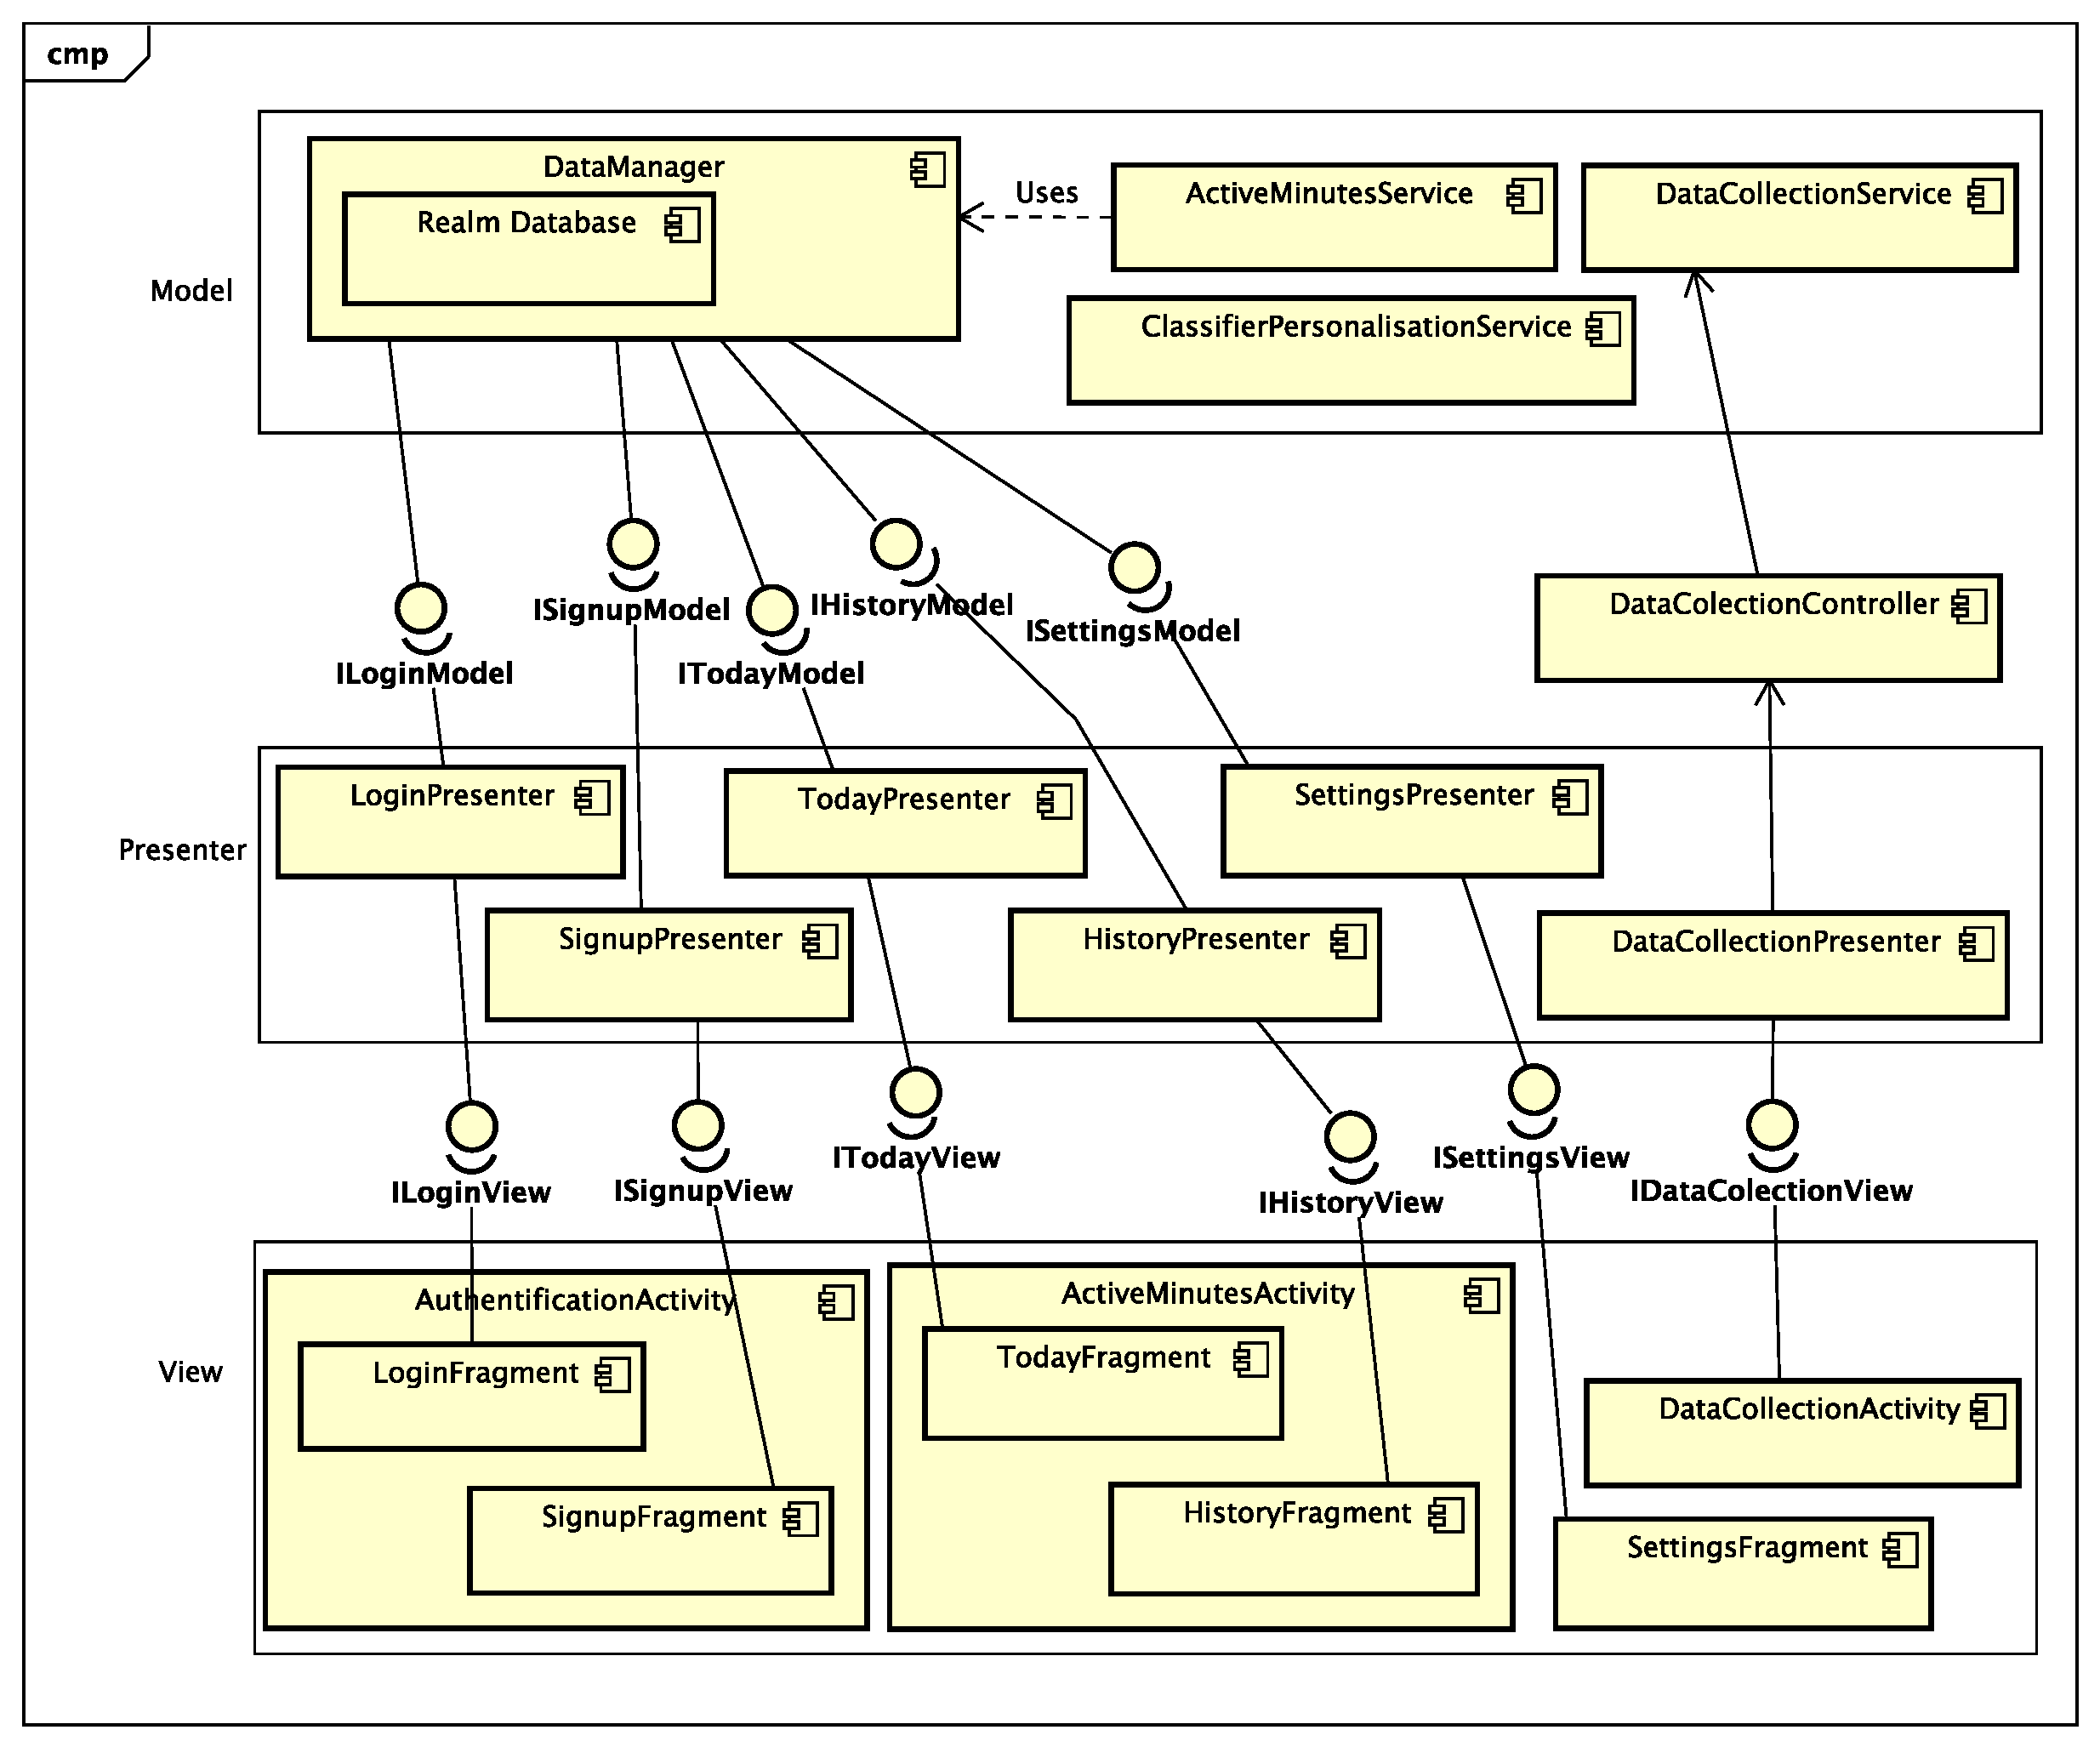
\includegraphics[width=15cm]{active-minutes-service-component-diagram}
        \caption{ \textit{"Active Minutes"} Architectural model (simplified)}
        \label{fig:architectural_design_component_diagram}
    \end{figure}
    
    Model-View-Presenter or \textbf{MVP} software architectural pattern was chosen to form the base of the proposed mobile system since it provides clean separation of concepts \citep[532]{zhang2010}. For example the \textit{View} represents the \gls{ui} of the application. It contains logic for receiving user interaction and notifying the \textit{Presenter}. The \textit{Model} is the data layer. It is responsible for providing and formatting (i.e. applying the business logic to) the data and returning it to the Presenter. The \textit{Presenter} acts as a mediator, it requests data from the \textit{Model} and returns it to update the \textit{View}. Figure \ref{fig:model_view_presenter_design_pattern} shows the interaction flow of the pattern. When the user interacts with the \gls{ui} of mobile application, the View receives the interaction (i.e. button click) and passes that information to the Presenter via Interface (\textit{IView}). The Presenter then invokes the appropriate method of the Model. Next, the Model returns the requested data to the View (via the Presenter). 
        
    The main \textbf{advantages} of using the \gls{mvp} pattern is that it increases the \textbf{testability} of the software via the concept of logic separation. For example, the View is only allowed to have framework specific code (i.e. Android UI components such as Button, ListView); Presenter and Model are comprised of Plain Old Java Objects or \textbf{POJO}. These POJO classes can be thoroughly tested outside the mobile application. In addition, the \gls{mvp} pattern introduces a certain level of abstraction in the software architecture via the use of Java Interfaces such as \textit{ILoginView} (see figure \ref{fig:architectural_design_component_diagram}). That allows different parts of the software to be developed separately and then integrated into the application. The components of the system will be discussed in the following sections.
    
    \begin{figure}[ht]
        \centering
        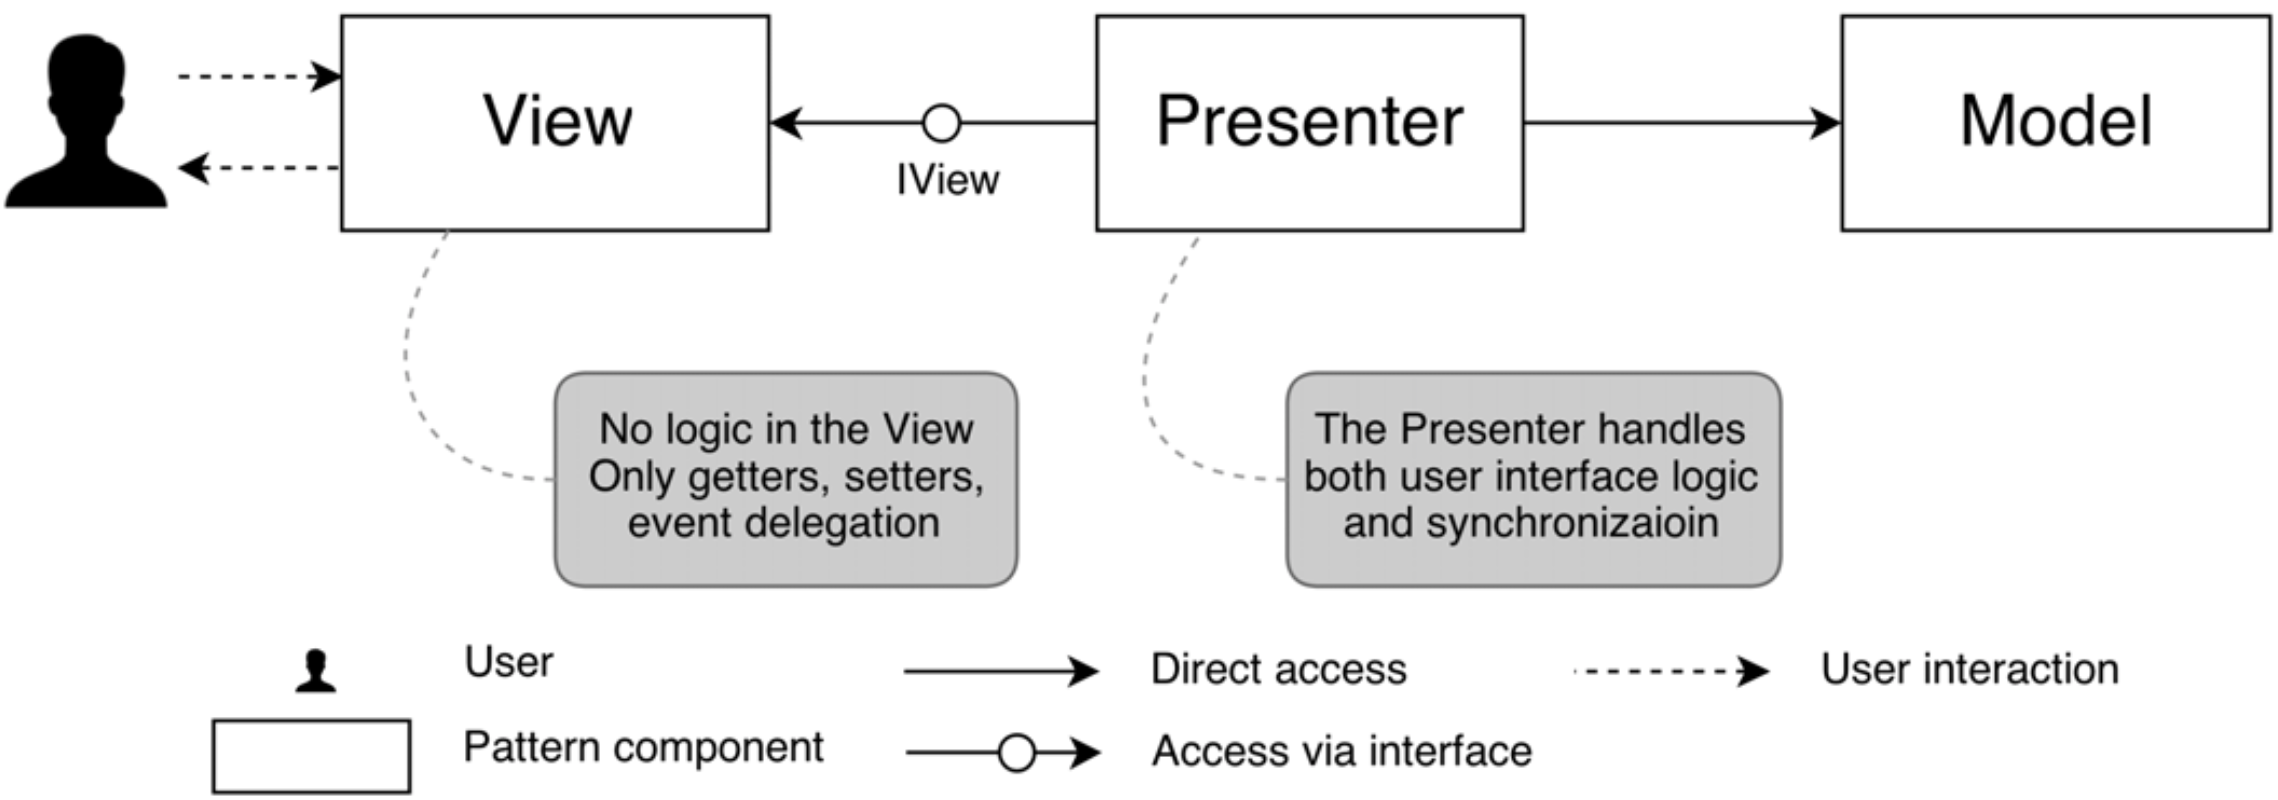
\includegraphics[width=15cm]{model-view-presenter-design-pattern}
        \caption{Model-View-Presenter design pattern \citep[28]{syromiatnikov2014}}
        \label{fig:model_view_presenter_design_pattern}
    \end{figure}
        
        \subsection{Models}
        As can be seen from figure \ref{fig:architectural_design_component_diagram} the \textit{Model} layer of the system architecture is comprised of \textit{DataManager}, \textit{ActiveMinutesService}, \textit{ClassifierPersonalisationService} and \textit{DataCollectionService}. These components will be discussed next.
        
            \subsubsection{DataManager}
            \label{section:data-manager}
            The \textbf{\textit{DataManager}}, as the name implies, is responsible for providing means of accessing the underling database object. For example, retrieving a list of activities for the logged-in user. Almost all of the diagram components have access to DataManager. Thus they can perform operations such as saving a new user or loading user's physical activity goal. This class essentially is a wrapper of a \textbf{Realm}\footnote{\url{https://realm.io/news/realm-for-android/}} database object. After initial research, \citet{realm2014} was chosen to form the database of the mobile application. It is a third-party Android library found to be x100 faster compared to the Android native SQLite Object-Oriented Data Management System (OMS).
            
            \subsubsection{ActiveMinutesService}
            \label{section:active-minutes-service}
            Since \textit{"Active Minutes"} has to collect contextual information throughout the user's day continuously, \textbf{\textit{ActiveMinutesService}} is implemented as an Android \textit{Service} class. According to \citet{googleservices2017}, a Service is an application component that continuously runs in the background even if the user closes or switches to another application. The responsibilities of this service include \gls{har}, storing the recognised activities in the database and performing additional checks such as whether or not to send reminder notification to the user for sitting for too long.
            
            Another important responsibility of the this service is to collect personal data. This data is used later on for classifier personalisation (e.g. adapting the general classifier so it better recognises user activities).
            
            \subsubsection{ClassifierPersonalisationService}
            \label{section:classifier-personal-service}
            The sole purpose of this service is to personalise the general classifier that is included in the application initially. The service is started by the above-mentioned \textit{ActiveMinutesService} service when enough labeled data is collected. For example, the service is executed when there are x100 instances of \textit{walking}, \textit{running}, \textit{cycling} and \textit{static} activity training data. Since it will run once in the lifetime of the application on the device, this service is implemented as a special kind of Service called \textit{IntentService}. It allows for executing heavy tasks such as training a classifier in a worker thread so the application's main UI thread is not affected.
            
            \subsubsection{DataCollectionService}
            \label{section:data_collection_service}
            In order to train a \gls{har} classifier, a training dataset is required. This service is responsible for the data collection process. That includes reading, prepossessing and windowing the raw accelerometer data as well as abstracting the data via the means of feature extraction (see section \ref{section:feature-selection&extraction}). Each feature vector stores 20 values (the first 5 \gls{fft} coefficients of every sensor axis, namely x,y and z and their magnitude) as a record in the \textit{Training\_data} table (see figure \ref{fig:data_modeling_er_diagram}).
            
        \subsection{Views}
        The View layer of the \gls{mvp} pattern is comprised of Interface classes that are implemented by Android components such as \textit{"Activity"} or \textit{"Fragment"}. This approach provides a layer of abstraction and logic separation which is one of the benefits of using the \gls{mvp} design pattern. From an Android standpoint, an \textit{Activity} is a class that creates a window (e.g. single screen) and its layout (a specific arrangement of \gls{ui} components such as \textit{"Buttons"}) can be set via using the method \textit{"setContentView(View)"} \citep{googleactivity2017}. According to \citet{googlefragments2017}, \textit{"Fragment"} is a \textit{"sub-activity"} like class with its own layout. They can be swapped with one another easily thus they are highly reusable. Fragments typically require a host Activity in order to be presented to the user. For example, the \textit{"LoginFragment"} and \textit{"SignupFragment"} are hosted in an Activity called \textit{"AuthenticationActivity"}. As it can be seen from figure \ref{fig:architectural_design_component_diagram} all of the \textit{View}s in the \gls{mvp} pattern communicate with a dedicated Presenter class in the \textit{Presenter} layer via an interface. The following sections will describe what are the responsibilities of each one of those components.
            
            \subsubsection{AuthenticationActivity}
            As the name of the component suggests, this is a Android \textit{Activity} class that handles the login and sign up functionality of the application. This activity is responsible of presenting the two fragments it hosts, namely \textit{"LoginFragment"} and \textit{"SignupFragment"}. The LoginFragment is responsible of checking the login user credentials and eventually transferring the user to the main screen of the mobile application. As for the SignupFragment, it handles the process of creating a new user.
            
            \subsubsection{ActiveMinutesActivity}
            The main purpose of this activity is to display the contents of the \textit{"TodayFragment"} (e.g. Today screen) and \textit{"HistoryFragment"} (e.g. History screen). The TodayFragment shows current information to the user such as how much time a user has been active today as well as details for the user's inactive time. The \textbf{HistoryFragment} is responsible for showing past activity information both daily and weekly. This way the user can refer to a previous day goal-performance.
            
            \subsubsection{DataCollectionActivity}
            This Android \textit{Activity} class is responsible for providing an interface for controlling the \textit{DataCollectionSertice} mentioned in section \ref{section:data_collection_service}. It's \gls{ui} provide buttons for starting and stopping the service as well as exporting the acquired data into a labeled dataset file format - \textit{ARFF}. Later on this file will be used to build a classifier using the machine learning library WEKA on the device itself.
            
            \subsubsection{SettingsFragment}
            As the name implies, this Fragment class is responsible for providing the user with the ability to change certain parameters of the application. For example, the user can change their \gls{pa} goal as well as \gls{st} goal. In addition, the user can change the the \textit{"Sleeping Hours"} time window and disable \gls{mci} reminding notifications.
            
            
        \subsection{Presenters}
        The \textit{Presenter} layer of application's architecture is comprised of a set of Presenter classes (see figure  \ref{fig:architectural_design_component_diagram}) needed for the different screens of the application. For example, the \textit{LoginFragment} (e.g. screen) has a presenter object \textit{LoginPresenter} which allows the screen to participate in the \gls{mvp} pattern e.g. communicate with the appropriate \textit{Model} and \textit{View} objects, namely \textit{ILoginView} and \textit{ILoginModel}.
    
    \section{Database Design}
    \label{section:database-design}
    This section discuses the design of the database system that will be used to store the data needed for the functionality of the mobile application. The design of the database can be seen in figure \ref{fig:data_modeling_er_diagram}. It includes the following entities \textbf{User}, \textbf{Activity} and \textbf{Training\_data}. The following sections will explain the responsibilities of each entity (i.e.\ database tables).
        
        \begin{figure}[ht]
            \centering
            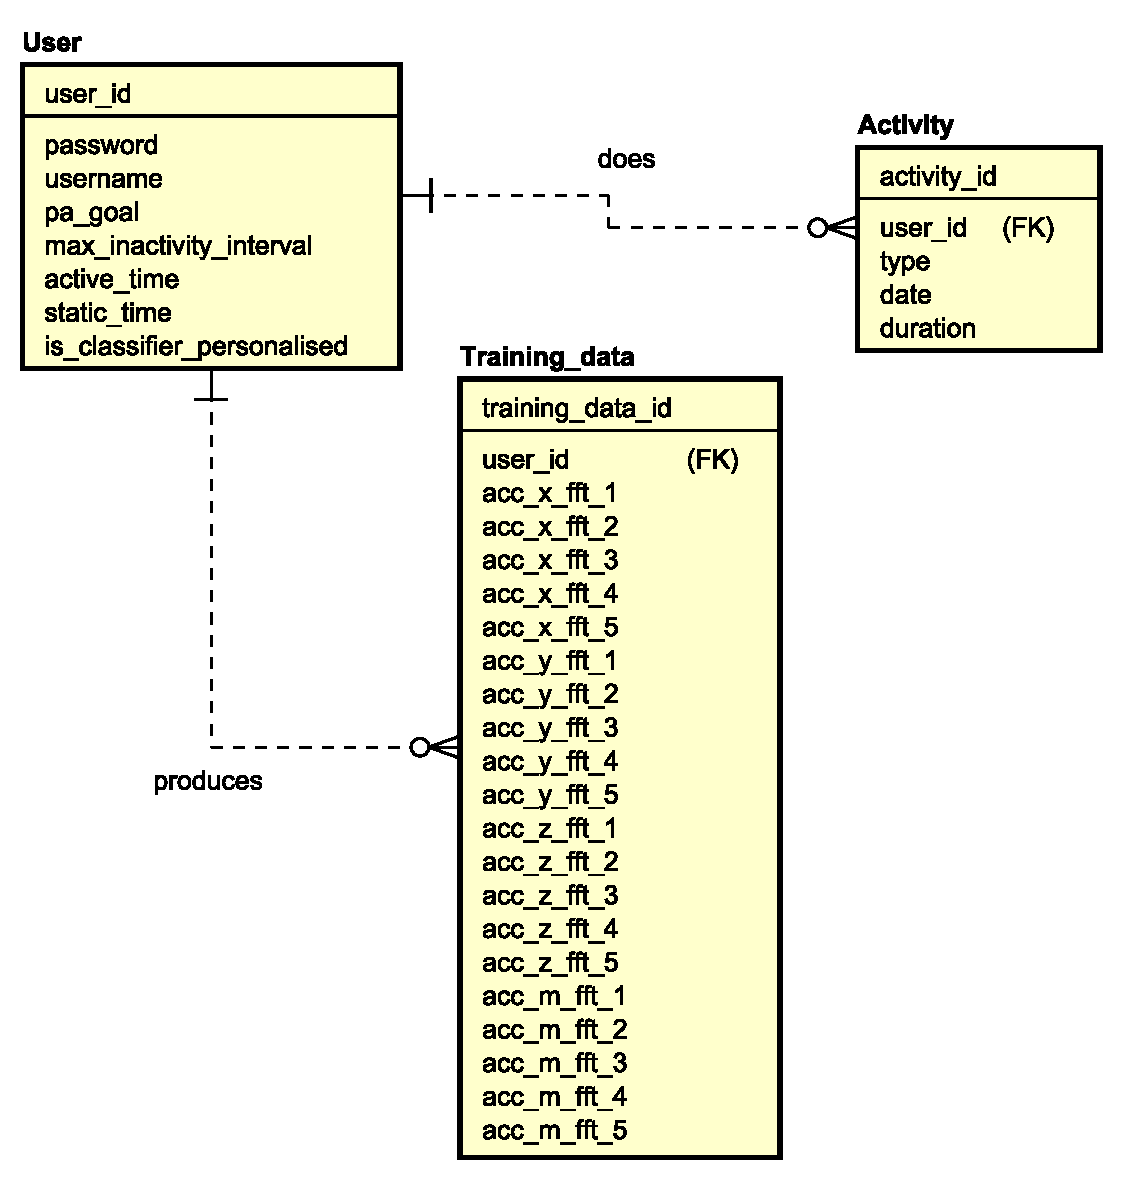
\includegraphics[width=12cm]{data-modeling-er-diagram}
            \caption{Database ER Diagram}
            \label{fig:data_modeling_er_diagram}
        \end{figure}
        
        \subsubsection{Entities}
        
        \begin{itemize}
            \item User(user\_id, password, username, pa\_goal,max\_cont\_inac\_goal, is\_classifier\_personalised, profile\_picture)
            \item Training\_data(user\_id, acc\_x\_fft\_1, acc\_x\_fft\_2, acc\_x\_fft\_3, acc\_x\_fft\_4...)
            \item Activity(activity\_id, user\_id, type, date, duration)
        \end{itemize}
        
        \subsubsection{Relationships}
        \begin{itemize}
        \item Does --- User does Activity [1:m][m:o]
        \item Produces --- User produces Training\_data [1:m][m:o]
        \end{itemize}
        
        \subsection{User}
        The user table is responsible for storing the personal information of every registered user. For example, \textbf{\textit{user\_id}} allows every user to be uniquely identified in the system. As for the \textbf{\textit{username}} and \textbf{\textit{password}} fields, they are used to authenticate different users of the application upon login.
        
        The user table stores additional information such as the \gls{pa} goal (\textbf{\textit{pa\_goal}}) and the maximum continuous inactivity goal (\textbf{\textit{max\_cont\_inac\_goal}}). The table also stores a Boolean field called \textbf{\textit{isClassifierPersonalised}}. This field is set to \textit{False} by default and only changed when the general classifier, bundled with the application, is personalised with user's data. Since every user sets their \textit{Sleeping Hours} by design (i.e. a time window during which the user would not be monitored) fields called \textit{startSleepingHours} and \textit{stopSleepingHours} are needed to store the start and stop sleeping hours set by the user. Last but not least, fields called \textbf{\textit{profile\_picture}} and \textbf{\textit{isFirstTime}} are responsible for storing the user's profile image and if the user uses the application for the first time, respectively.
        
        \subsection{Activity}
        As it can be seen from figure \ref{fig:data_modeling_er_diagram}, the Activity table is responsible for storing information for the different activities. Every table record is created for every day of the week. Once created, its fields are amended accordingly throughout the day depending on the \gls{pa} and \gls{st} levels. 
        
        Every activity record in the table has a unique identifier \textbf{\textit{activity\_id}} that uniquely identifies it. Also, the table stores the user's id in a field called \textbf{\textit{user\_id}}. That allows for associating a given activity record with a specific user.
        
        The table is also storing fields that store user's activity levels. For example, \textbf{\textit{active\_time}} field stores the amount of \gls{pa} the user is accumulated for a specific day. Other table fields are responsible to storing statistical information regarding sedentary information such as \textit{longest\_inactivity\_interval}, \textit{currentInactivityInterval}, \textit{averageInactivityInterval} and \textit{totalInactivityTime}. In addition, a field called \textit{timesCurrentInactivityReset} is used to store how many times the current inactivity is being reset (needed to calculate the average inactivity interval). A reset happens when an activity of type \textit{Active} is recognised by the classifier. Consequently, the \textit{currentInactivityInterval} is reset to zero and \textit{timesCurrentInactivityReset} incremented.
        
        \textbf{\textit{Activity}} table also stores user's \gls{pa} goal, represented by \textit{user\_pa\_goal} as well as \gls{st} goal represented by \textit{user\_max\_cont\_inac\_goal}.
        
        \subsection{Training\_data}
        The last database table to discus is the Training\_data. The fields from the table \textbf{\textit{acc\_x\_fft\_1}},\newline\textbf{\textit{acc\_x\_fft\_2}},\textbf{\textit{acc\_x\_fft\_3}}... are responsible for storing the extracted features from the raw accelerometer data as discussed in section \ref{section:proposed-application}. The table field \textbf{\textit{user\_id}} is used to associate a user with a particular record in the table. \textit{ClassValue} field stores the label of the training data record (i.e. walking or static).
        
        One point to note, this table is used for two purposes at different times of the development of the project. Firstly, it is used during the application development to store all of the project participants training data. This data will be used to build a general classifier. Secondly, this table is used as part of the final solution to store labeled data needed to build a personalised classifier for a particular user.
    
    
        
    \section{User Interface Design}
    \label{section:user_interface_design}
    The process of designing the user interface is highly dependent on the system's specifications discussed in chapter \ref{Chapter:Specification}. For example, the application requires user authentication thus a design for the log-in and sign-up screens have been developed. A \gls{ui} design process proposed by \citet[60]{bell2005} has been applied in this work (see figure \ref{figure:ui-design-process}). According to Bell, the \gls{ui} design process is usually informed by certain design principles and guidelines to make sure that the application is user-friendly. Next, prototyping tools are used to create a system prototype which is evaluated by the user for quality. That is followed by integrating the client's feedback into the prototype. This process is repeated until the client is happy with the prototype of the system. The following sections discuss how the mobile application \gls{ui} has been developed as well as what design principles and guidelines were considered during this process.
    
    \begin{figure}[ht]
    \centering
        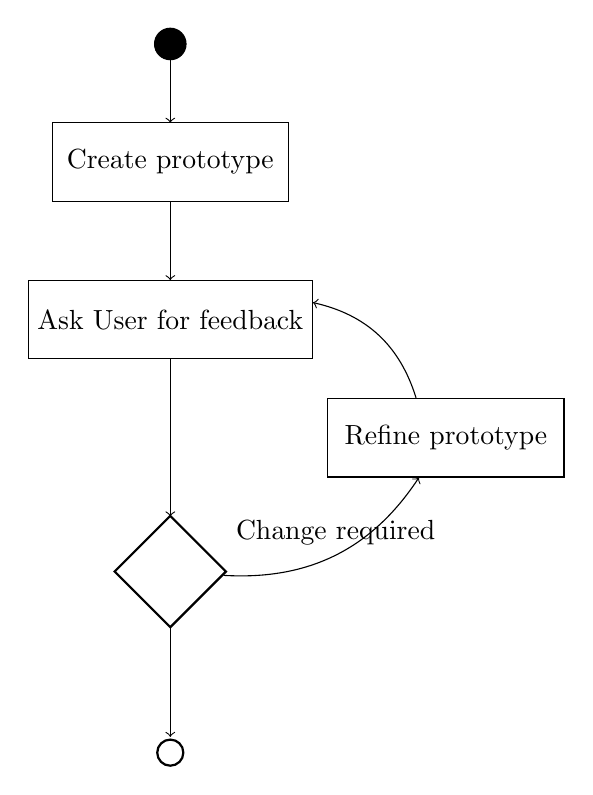
\begin{tikzpicture}
            \draw[fill=black] (0,0) circle (0.2);
            \draw [->] (0,0) -- (0,-1);
            \draw (-1.5,-1) rectangle (1.5,-2);
            \node at (0,-1.5) {Create prototype};
            
            \draw [->] (0,-2) -- (0,-3);
            \node (check) [draw, shape=rectangle, minimum width=2.5cm, minimum height=1cm, anchor=center] at (0,-3.5) {Ask User for feedback};
            
            \draw [->] (0,-4) -- (0,-6);
            \node (usercheck) [draw, thick, shape=rectangle, minimum width=1cm, minimum height=1cm, anchor=center,rotate=45] at (0,-6.7) {};
            
            \node (ref) [draw, shape=rectangle, minimum width=3cm, minimum height=1cm, anchor=center] at (3.5,-5) {Refine prototype};
            
            \draw [->] (0,-7.4) -- (0,-8.8);
            \node (end) [draw, thick, shape = circle, minimum width = 0.3cm] at (0,-9) {};
            
            \draw[->, to path={-| (\tikztotarget)}]
            (ref) edge[bend right] node [left] {} (check) 
            (usercheck) edge[bend right] node [pos=.5,above] {Change required} (ref);
            
        \end{tikzpicture}
    \caption{Iterative process of UI prototyping}
    \label{figure:ui-design-process}
    \end{figure}
    
        \subsection{System Prototyping}
        In order to create the system prototype, a set of wireframes were created (see appendix \ref{chapter:screen-wireframes}). Next, the wireframes were further developed into a \gls{ui} design. Both the wireframe and user interface designs were created using a professional software design tool \textit{Sketch}\footnote{\url{https://www.sketchapp.com/}}. The design of every mobile screen implemented in mobile application the can be seen in appendix \ref{chapter:screen-design}. 
        
        When the initial versions of all mobile screen UI design were finished, a software called \textit{Flinto}\footnote{\url{https://www.flinto.com/}} was used to create a system prototype. One of the reasons of choosing \textit{Sketch} as a design tool is because it allows for easy export of Sketch pages to \textit{Flinto} documents thanks to a dedicated plugin.
        
        In order to create the prototype, special objects called \textit{Links} had to be drawn over the mobile screen designs . Every link needs a target to be specified. For example, in figure \ref{fig:flinto_prototype}) there is a link object drawn over the \textit{"Weekly"} button and its target is set to be the whole \textit{"History Screen Weekly"} screen. So when the client inspects the design prototype and presses the \textit{Weekly} button they will be taken to the weekly view page. This process of creating links and targets was used for all UI screen designs to create a functioning system prototype that the client can interact with and gain a clearer idea of how the system will be implemented and share valuable feedback.
        
        \begin{figure}[ht]
            \centering
            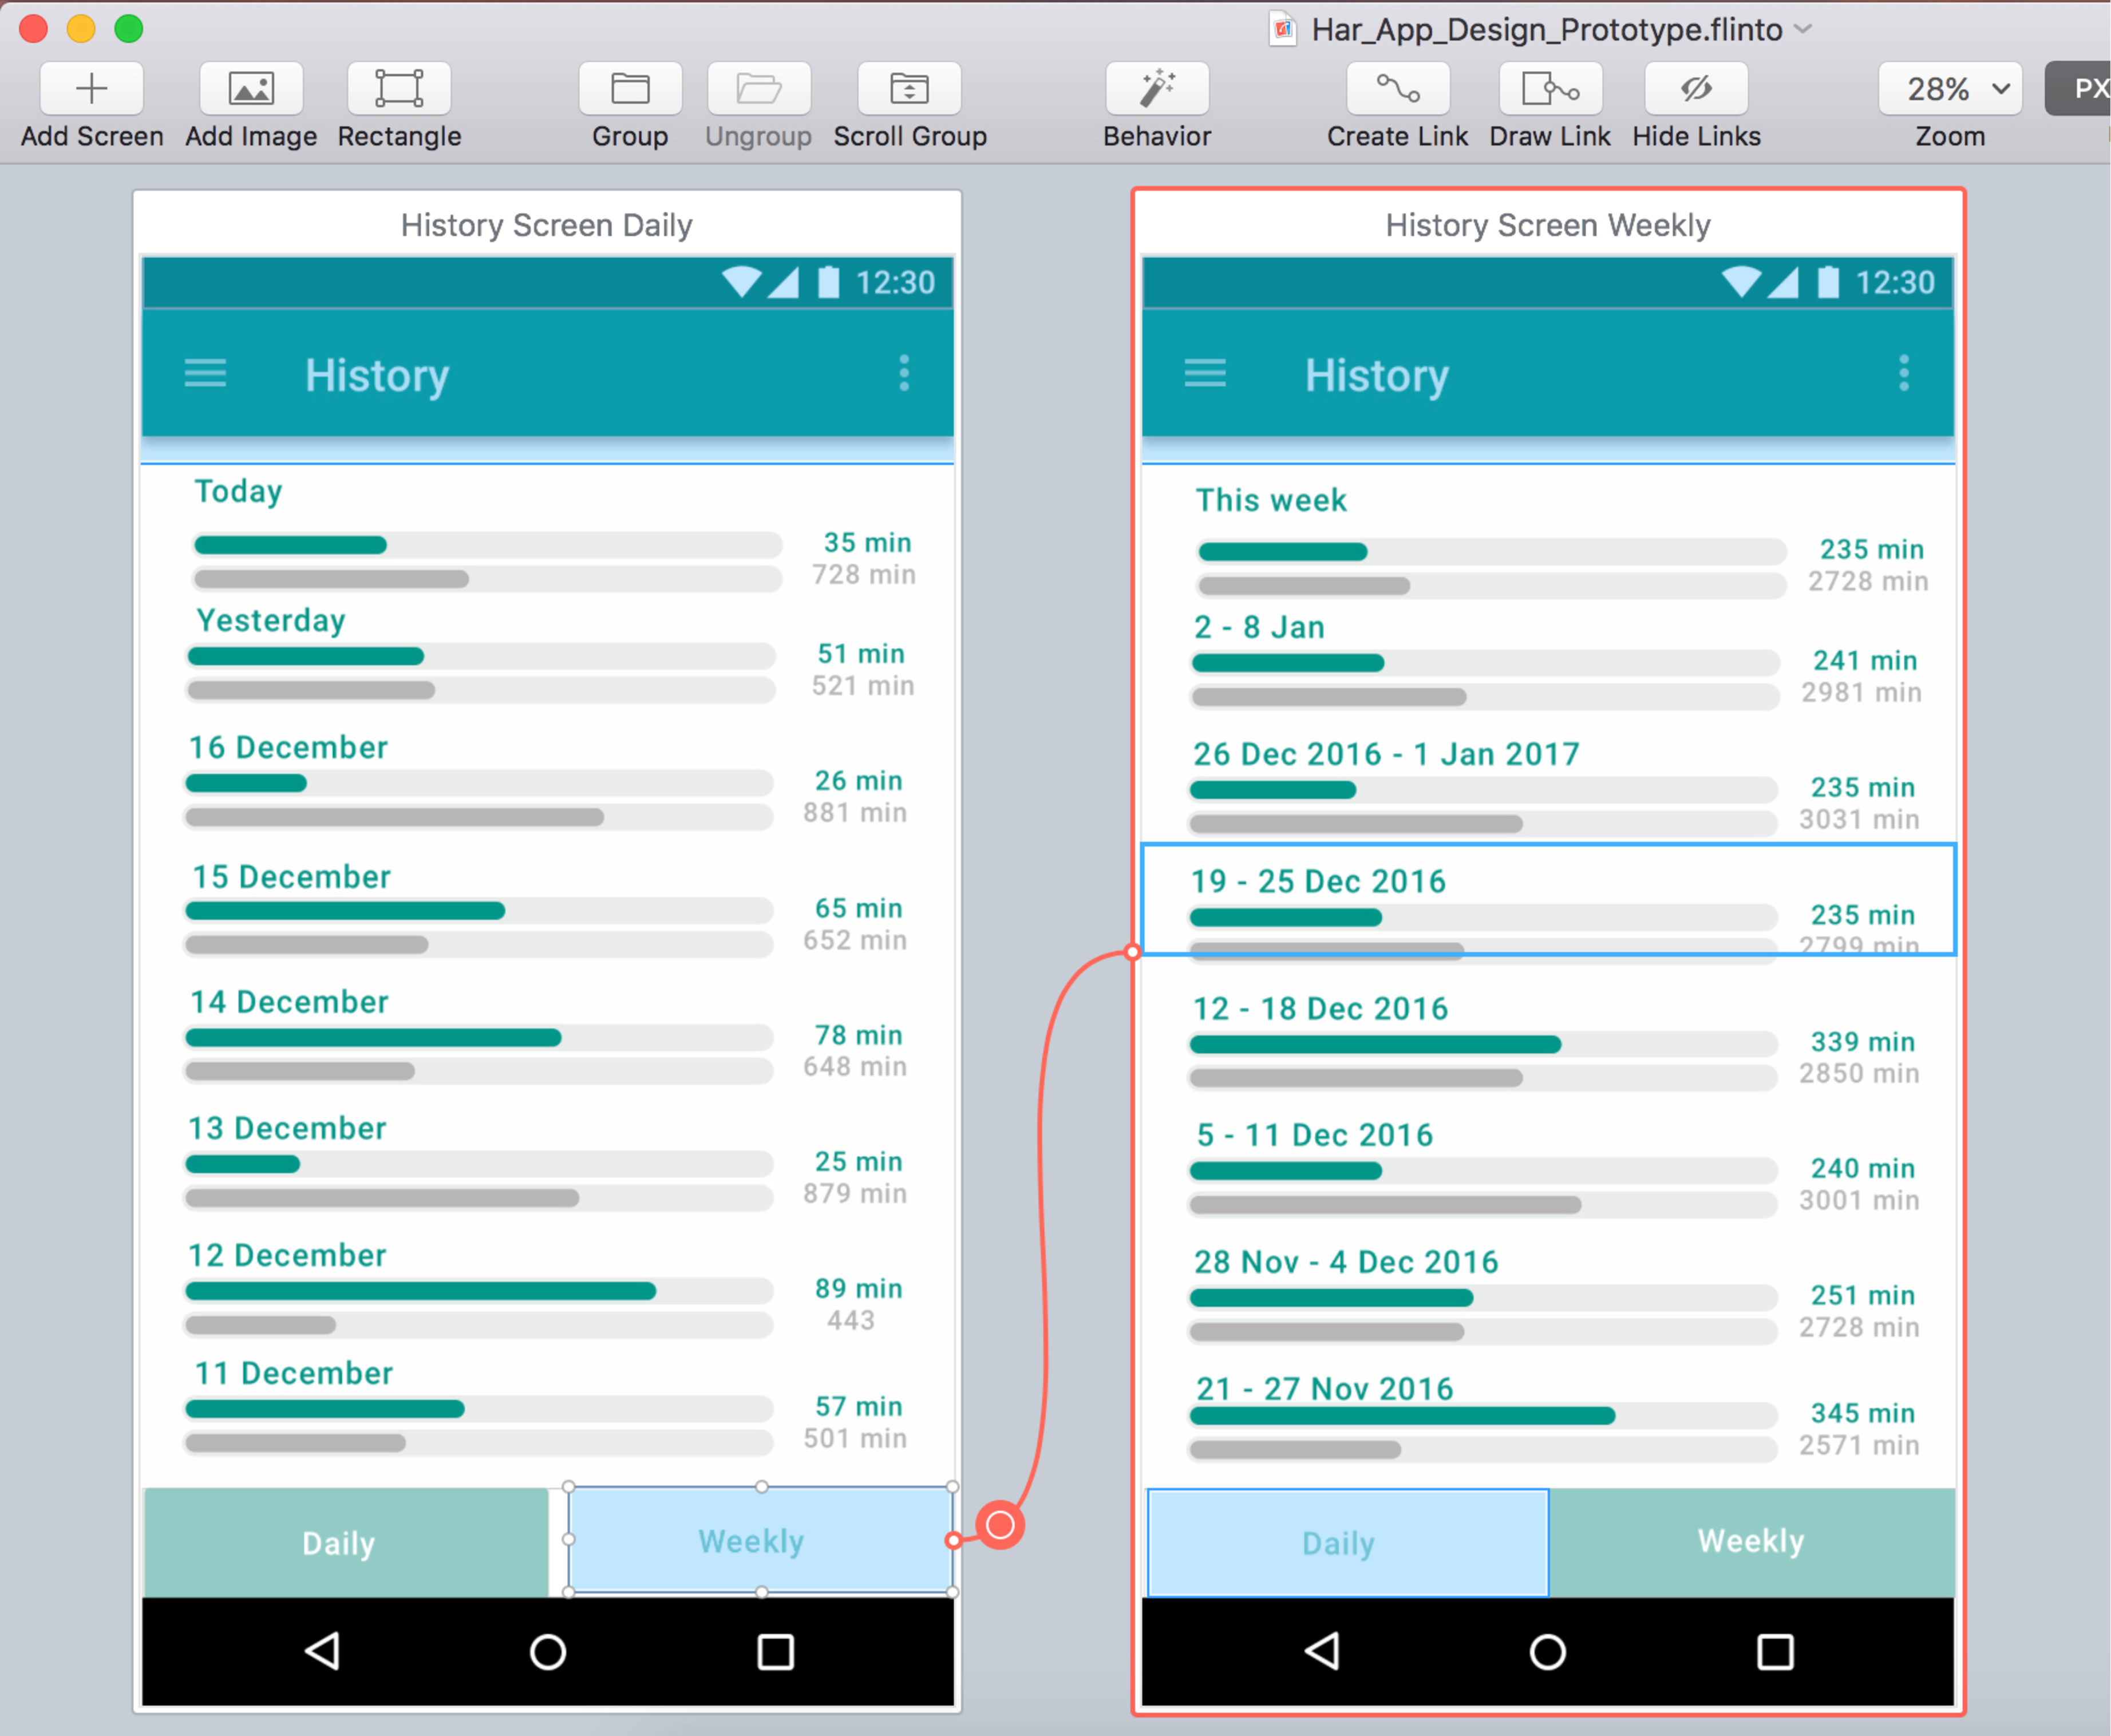
\includegraphics[width=12cm]{flinto-screen-links}
            \caption{Flinto prototype creation process}
            \label{fig:flinto_prototype}
        \end{figure}
        
        
        \subsection{Design Principles and Guidelines}
        
        \subsubsection{Design Principles}
        Design principles are well-accepted principles that can inform how a user interface is being designed. Platform specific principles have informed the system design. For example, the first design principle suggested by \citet{google2017b} \textbf{"Delight me in surprising ways"} have been implemented in the authentication screens as the ability of the user to change screens via a swipe gesture. This action is reflected by the \textit{page indicator} at the bottom of the screens (see figure \ref{fig:authentication-screens}). According to Google, subtle effects such as these contribute to a feeling of effortless. 
        
        \textbf{"Only show what I need when I need it"} is another principle suggested by \citet{google2017b}. It focuses on the fact that people get confused when presented with a lot of information at once. \textit{"Active Minutes"} incorporates this principle by providing a \textit{"Navigational Drawer"} that provides additional options for the user such as \textit{"Settings"} and \textit{"Log Out"}. When not needed, the drawer can be closed (see figure \ref{fig:nav-drawer-opened}). 
        
        \textbf{"I should always know where I am"} is a principle that allows the user to gain confidence that they know how how to use the system. For example, when switching between the \textit{Login} and \textit{Signup} screens the text of the button is changed to \textit{"LOG IN"} and \textit{"SIGN UP"} accordingly so the user can infer where they are at the moment (see figure \ref{fig:authentication-screens}).
        
        As per system specifications, the system will notify the user when a goal is met (see section \ref{section:feedback-component}). The next principle \textbf{"Only interrupt me if it's important"} implies that the user should not be interrupted unless it is important. For example, the system sends a notification when a prolonged sedentary time is recognised. In this case, the user must be notified so they can take action.
        
        \subsubsection{Design Guidelines}
        \citet[57-59]{bell2005} states that Design Guidelines need to be considered in the context of the platform the software is being designed for. Since \textit{"Active Minutes"} is developed as an Android application, it needs to comply with the platform specific design guidelines. That is why the system design has been informed by the official Android design guidelines \citep{googleamaterialdesign}. Google's new design language called \textit{"Material Design"} have been applied to the design of the application. It provides various guidelines such as the ideal layout metrics to be used when designing a \textit{Navigation Drawer}. 